\documentclass[runningheads]{llncs}

\usepackage[T1]{fontenc}
\usepackage[expansion=false]{microtype}
\usepackage{amsmath,amssymb,amsfonts}
\usepackage{graphicx}
\usepackage{textcomp}
\usepackage{booktabs}
\usepackage{multirow}
\usepackage{array}
\usepackage{subcaption}
\usepackage{url}
\usepackage[hidelinks]{hyperref}

\graphicspath{{figures/}}

\setlength{\textfloatsep}{8pt plus 2pt minus 2pt}
\setlength{\intextsep}{8pt plus 2pt minus 2pt}
\setlength{\abovecaptionskip}{4pt}
\setlength{\belowcaptionskip}{2pt}

\newcolumntype{L}[1]{>{\raggedright\arraybackslash}p{#1}}
\newcolumntype{C}[1]{>{\centering\arraybackslash}p{#1}}

\begin{document}

\title{Equal Accuracy, Different Mistakes: Classifier Heads and\\Error
Diversity in Fine-Grained Waste Classification}

\titlerunning{Equal Accuracy, Different Mistakes}

\author{Minhhoang Le \and Vanha Tran}
\authorrunning{M. Le and V. Tran}
\institute{Faculty of Artificial Intelligence, FPT University, Hanoi 155514, Vietnam\\
\email{hatv14@fe.edu.vn}}

\maketitle

\begin{abstract}
Transfer learning studies in image classification usually vary the backbone,
report the best test accuracy, and stop there. We argue that this hides most of
what the experiment actually measured. We train all 18 combinations of six
ImageNet-pretrained backbones and three classifier heads on a 36-class waste
image dataset, repeat every combination under two random seeds, and then look
at per-image predictions rather than at summary scores. Three things follow.
First, the choice of head behaves far more consistently than the choice of
backbone: a global-average-pooling head with batch normalisation and dropout
beats a plain linear head on all six backbones under both seeds, and the
train--test gap grows monotonically with head capacity, from 3.6 points to 7.3
points on average. Second, of the 153 model pairs, 57 cannot be separated by
McNemar's test, yet those same pairs disagree on 437 test images on average.
Equal accuracy does not mean equal errors. Third, we exploit that: across all
816 three-model soft-voting ensembles, the mean accuracy of the members
explains almost none of the gain over the best member ($R^2 = 0.001$), while
adding their mean pairwise disagreement raises $R^2$ to 0.29, with a large and
highly significant diversity coefficient. Both predictors are measured on a
held-out validation split and the gain on test, so no test information enters
the selection. The practical consequence is narrower than the statistical one.
Rules that maximise diversity directly do not survive this honest protocol:
their apparent advantage shrinks by about two points once diversity is
estimated off the test set. What does survive is the cheap structural proxy: taking one model per backbone
beats a random selection of the same size at every ensemble size from two to
six, under both seeds.

\keywords{Ensemble diversity \and Transfer learning \and Classifier head
\and Model selection \and Waste classification}
\end{abstract}

\section{Introduction}

A large part of applied image classification now consists of the same recipe:
take a network pretrained on ImageNet, replace its final layer, fine-tune on
the target data, and report the test accuracy of whichever variant came out on
top. The recipe works. It is also a weak experiment, because almost everything
it measures is thrown away. A single accuracy figure per model cannot say
whether two models that scored 90.0\% and 90.1\% are doing the same thing, and
it cannot say whether the 0.1 point between them is a finding or noise.

This paper works with the discarded information. We fix one task --- 36-class
fine-grained waste classification, where classes are visually similar and
severely imbalanced --- and train a full grid of six backbones crossed with
three classifier heads, twice, under two random seeds. That gives 36 trained
models, 18 configurations with a replicate each. We then analyse the per-image
predictions directly.

Our interest is not in which configuration wins. It is in three questions that
a leaderboard cannot answer:

\begin{itemize}
\item \textbf{Which design choice is stable?} The field tunes backbones and
treats the classifier head as an afterthought. We find the opposite ordering:
the head effect is consistent across every backbone and both seeds, while the
backbone ranking moves between seeds.
\item \textbf{What does statistical equality hide?} When a significance test
says two models are indistinguishable, practitioners read that as "either one
will do". We show that these pairs still disagree on several hundred images,
and that the disagreement is the useful part.
\item \textbf{What should drive ensemble member selection?} The standard answer
is to ensemble the best models. We test this exhaustively over all 816 possible
three-model ensembles and find that member accuracy is close to useless as a
predictor of ensemble gain, while pairwise disagreement is not.
\end{itemize}

The contribution is an analysis, not an architecture. We use a waste dataset
because it is a realistic fine-grained, long-tailed problem, not because the
method is specific to waste.

\section{Related Work}

\paragraph{Transfer learning for waste classification.}
ImageNet-pretrained convolutional networks are the standard tool here.
Vo et al.~\cite{vo2019novel} reach 94\% on TrashNet with a ResNeXt-based model,
Feng et al.~\cite{feng2022intelligent} reach 94.23\% with a simplified MBConv
block and added attention, and Zhang et al.~\cite{zhang2021} add a
self-monitoring module to ResNet18. These share a pattern: a new backbone or
backbone modification, a small dataset with few classes, a single run. On
larger label sets, Sayem et al.~\cite{sayem2025enhancing} reach 83.11\% over 28
recyclable categories, and Nahiduzzaman et al.~\cite{nahiduzzaman2025automated}
reach 85.25\% on the 36-class task we use, with the TriCascade dataset they
introduce. Accuracy drops sharply as the number of similar classes grows, which
makes this setting useful for studying errors rather than headline scores.

\paragraph{Classifier heads.}
The layers between a frozen feature extractor and the softmax receive little
systematic attention. Most papers state the head in one sentence and vary
something else. We are not aware of a study that crosses several heads with
several backbones on the same protocol and asks whether the head effect is
stable. Our results suggest it is the more reliable of the two axes.

\paragraph{Ensemble diversity.}
That ensemble members should make different errors is an old idea. Kuncheva and
Whitaker~\cite{kuncheva2003measures} catalogue ten diversity measures and
examine how they relate to ensemble accuracy, reporting that the relationship
is weaker and less consistent than intuition suggests. Dietterich's
survey~\cite{dietterich2000ensemble} frames diversity as a precondition for
ensembling to help at all. In deep learning, Lakshminarayanan et
al.~\cite{lakshminarayanan2017simple} show that independently initialised
networks form strong ensembles, and Fort et al.~\cite{fort2019deep} attribute
this to the members landing in different modes of the loss landscape.
Gontijo Lopes et al.~\cite{gontijolopes2022one} show that models trained with
different recipes make substantially different errors even at matched accuracy.

Those studies vary initialisation or training recipe while holding architecture
fixed. We do the opposite, which is the situation a practitioner is in when
choosing among several fine-tuned candidates, and we test the resulting
selection rules exhaustively rather than on hand-picked combinations.

\section{Experimental Setup}

\paragraph{Data.}
We use the Stage 3 subset of the TriCascade WasteImage
dataset~\cite{tricascade_dataset,nahiduzzaman2025automated}, which labels 35{,}264
real-world waste photographs with 36 fine-grained categories. The classes are
visually close --- cigarette butts against syringes, spray cans against beverage
cans, plastic cups against paper cups --- and heavily imbalanced, with a
54.9:1 ratio between the largest and smallest class. All images were re-encoded
with OpenCV to strip metadata and standardise the format; unreadable files were
dropped.

We use a stratified 80/10/10 split: 28{,}201 training, 3{,}511 validation and
3{,}552 test images. The test set is held out and never used for model
selection. Augmentation (horizontal flip, small rotation, zoom, brightness,
translation and contrast jitter) is applied online during training only.

\paragraph{Configurations.}
We cross six ImageNet-pretrained backbones with three classifier heads. The
backbones are EfficientNetV2B0~\cite{tan2021efficientnetv2},
MobileNetV3Small~\cite{howard2019mobilenetv3}, ResNet50~\cite{he2016resnet},
DenseNet201~\cite{huang2017densenet},
InceptionV3~\cite{szegedy2016inceptionv3} and
Xception~\cite{chollet2017xception}. The heads are:

\begin{itemize}
\item \textbf{SIMPLE\_FC}: global average pooling, batch normalisation, dropout
(0.5), softmax. The minimal head.
\item \textbf{GAP\_BN\_FC\_Drop}: as above plus a 512-unit ReLU layer with its
own batch normalisation and dropout before the softmax.
\item \textbf{DUAL\_POOLING\_FC}: average and max pooling in parallel, batch
normalisation, then a residual block with a 512-unit projection shortcut added
to a parallel 512-unit ReLU branch (dropout 0.4), then softmax. The largest head.
\end{itemize}

The original classification top is removed in every case, and the only
difference between configurations is the backbone and the head. Images are
resized to each backbone's native input ($224\times224$, or $299\times299$ for
InceptionV3 and Xception) and passed through that backbone's own preprocessing
function.

\paragraph{Training.}
Every configuration follows the same two-stage schedule. The backbone is first
frozen for three warm-up epochs at learning rate $1\times10^{-3}$ so that the
new head settles before it can push large gradients into pretrained weights.
The whole network is then unfrozen and fine-tuned for up to 30 epochs at
$1\times10^{-5}$. Given the class imbalance we use balanced class weights and
focal loss instead of plain cross-entropy. Learning rate is reduced on plateau
(factor 0.3, patience 3) and early stopping with patience 5 selects the best
epoch by validation accuracy. Training used TensorFlow 2.19 on a single NVIDIA
Tesla P100 with batch size 32.

\paragraph{Replication.}
Every configuration was trained twice, under seeds 36 and 42, giving 36 models
in total. We report both seeds throughout and treat a result as real only if it
holds under each. Two seeds bound the run-to-run variation but do not estimate
it precisely; we return to this in Section~\ref{sec:limits}.

\section{The Head Is the Stable Axis}

Table~\ref{tab:main} gives test accuracy for all 18 configurations under both
seeds, together with training accuracy and the resulting train--test gap.

\begin{table}[tb]
\centering
\caption{Test accuracy (\%) for all 18 configurations under two seeds. Best in
each column in bold. Training accuracy and the resulting train--test gap are
shown in Fig.~\ref{fig:gap}.}
\label{tab:main}
\begin{tabular}{llrrr}
\toprule
Backbone & Head & seed 36 & seed 42 & mean \\
\midrule
EfficientNetV2B0 & SIMPLE\_FC        & 88.99 & 89.25 & 89.12 \\
EfficientNetV2B0 & GAP\_BN\_FC\_Drop & 90.03 & 90.23 & 90.13 \\
EfficientNetV2B0 & DUAL\_POOLING\_FC & \textbf{90.71} & 90.43 & \textbf{90.57} \\
DenseNet201      & SIMPLE\_FC        & 87.89 & 89.08 & 88.49 \\
DenseNet201      & GAP\_BN\_FC\_Drop & 89.58 & 90.01 & 89.79 \\
DenseNet201      & DUAL\_POOLING\_FC & 90.17 & \textbf{90.54} & 90.36 \\
Xception         & SIMPLE\_FC        & 88.80 & 88.01 & 88.40 \\
Xception         & GAP\_BN\_FC\_Drop & 89.47 & 89.92 & 89.70 \\
Xception         & DUAL\_POOLING\_FC & 88.96 & 89.05 & 89.01 \\
ResNet50         & SIMPLE\_FC        & 87.75 & 87.50 & 87.63 \\
ResNet50         & GAP\_BN\_FC\_Drop & 88.91 & 88.85 & 88.88 \\
ResNet50         & DUAL\_POOLING\_FC & 88.68 & 88.54 & 88.61 \\
InceptionV3      & SIMPLE\_FC        & 87.39 & 86.99 & 87.19 \\
InceptionV3      & GAP\_BN\_FC\_Drop & 88.12 & 88.77 & 88.44 \\
InceptionV3      & DUAL\_POOLING\_FC & 88.03 & 87.64 & 87.84 \\
MobileNetV3Small & SIMPLE\_FC        & 82.88 & 82.66 & 82.77 \\
MobileNetV3Small & GAP\_BN\_FC\_Drop & 85.59 & 84.80 & 85.19 \\
MobileNetV3Small & DUAL\_POOLING\_FC & 86.18 & 85.11 & 85.64 \\
\bottomrule
\end{tabular}
\end{table}

\paragraph{The head effect is consistent; the backbone effect is not.}
Adding one hidden layer to the head (GAP\_BN\_FC\_Drop over SIMPLE\_FC) improves
accuracy on all six backbones under both seeds --- twelve out of twelve
comparisons, by between 0.68 and 2.70 points. A paired Wilcoxon signed-rank test
over those twelve pairs gives $W = 0$, $p = 4.9\times10^{-4}$.

The backbone ranking is less dependable. EfficientNetV2B0 leads under seed 36
and DenseNet201 under seed 42, and the two are separated by 0.21 points in the
seed-averaged column. Reporting either as "the best backbone" from a single run
would be reading noise. The head conclusion survives replication; the backbone
conclusion does not.

\begin{figure}[tb]
\centering
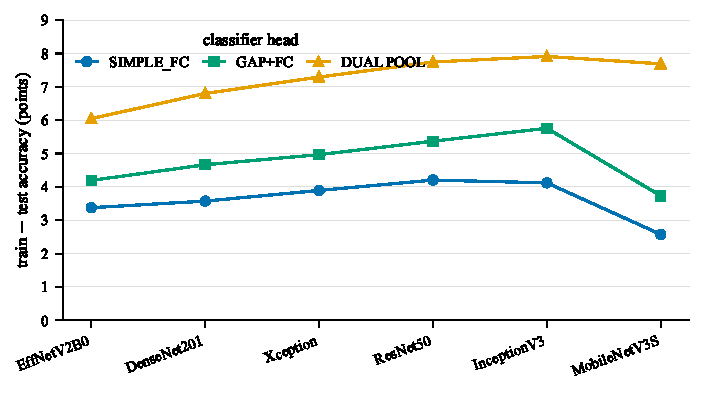
\includegraphics[width=0.70\textwidth]{fig1_head_gap.pdf}
\caption{Train--test gap by backbone and classifier head (seed 36). The three
heads separate cleanly and in order of capacity on every backbone, while test
accuracy for the two larger heads is nearly tied. The extra parameters in
DUAL\_POOLING\_FC are spent on the training set.}
\label{fig:gap}
\end{figure}

\paragraph{Head capacity buys training accuracy, not test accuracy.}
The train--test gap is more informative than accuracy here
(Fig.~\ref{fig:gap}). Averaged over backbones, the gap is 3.63 points for
SIMPLE\_FC (range 2.58--4.21), 4.78 for GAP\_BN\_FC\_Drop (3.73--5.76) and 7.25
for DUAL\_POOLING\_FC (6.05--7.92). The ordering is monotonic in head capacity
and holds for every backbone individually. The DUAL\_POOLING\_FC range does not
overlap either of the others.

Yet in mean test accuracy the two larger heads are nearly tied (88.79 and 88.62
under seed 36; 88.55 and 88.76 under seed 42). The extra capacity in
DUAL\_POOLING\_FC is spent almost entirely on fitting the training set. This is
a cleaner statement than "the medium head is best", and it is only visible
because the gap was measured for every cell of the grid rather than for the
winner alone.

\section{Statistical Equality Hides Different Errors}

We next ask what the accuracy column leaves out. For each of the
$\binom{18}{2} = 153$ model pairs within a seed we run McNemar's
test~\cite{mcnemar1947note,dietterich1998approximate} on the paired
correct/incorrect outcomes, using the exact binomial form when fewer than 25
discordant cases are available.

Under seed 36, 57 of the 153 pairs cannot be separated at $p > 0.05$; under seed
42, 41 pairs. The usual reading is that these models are interchangeable.

\begin{figure}[tb]
\centering
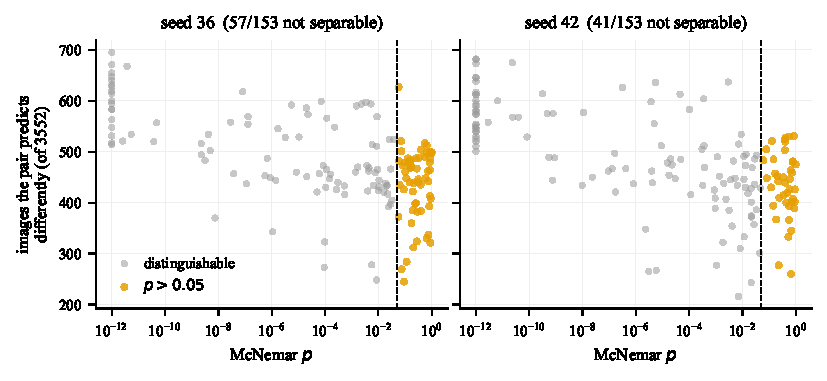
\includegraphics[width=0.84\textwidth]{fig2_mcnemar.pdf}
\caption{Every model pair, plotted by McNemar $p$-value against the number of
test images on which the two models predict different labels. Pairs to the
right of the dashed line are statistically indistinguishable, yet none of them
agrees on fewer than 245 images. The two axes are close to independent:
knowing that a significance test cannot separate two models says almost nothing
about how similarly they behave.}
\label{fig:mcnemar}
\end{figure}

They are not (Fig.~\ref{fig:mcnemar}). The indistinguishable pairs disagree on an average of 437 test
images under seed 36 (range 245--627) and 436 under seed 42 (range 260--531).
That is 12\% of the test set. Of those pairs, both models are simultaneously
wrong on only 230 images on average under seed 36 and 220 under seed 42. In
other words, a large share of the errors made by one member of an
indistinguishable pair is corrected by the other.

McNemar's test is answering the question it was asked --- whether one model is
more often right than the other --- and answering it correctly. The point is
that this is the wrong question if the goal is to combine models. Two models
can be equally accurate and still be highly complementary, and nothing in the
accuracy column indicates which case you are in.

\section{Diversity Predicts Ensemble Gain, Accuracy Does Not}
\label{sec:diversity}

If the errors of similar-accuracy models are complementary, combining them
should pay. We test this exhaustively. For each seed we form all
$\binom{18}{3} = 816$ three-model soft-voting ensembles by averaging the
predicted class probabilities, with no retraining and no weighting.

\paragraph{Protocol.}
Everything a practitioner would use to choose members is measured on the
held-out validation split: member accuracy, pairwise disagreement, and the
identity of the best single model. Only the final ensemble accuracy is measured
on test. This matters. Estimating diversity on the test set and then selecting
on it, as is common in the ensemble literature, lets the selection rule fit the
test set; Section~\ref{sec:select} shows that the difference is large enough to
reverse a conclusion. Validation and test accuracy are strongly but not
perfectly related across the 18 models ($r = 0.970$ for seed 36, $r = 0.986$
for seed 42), so the substitution is not free.

Ensembling helps almost always, but not uniformly. Under seed 36, 730 of the
816 triples (89\%) beat their best member, and 738 of 816 under seed 42. The
best triple reaches 93.38\% and 93.36\%, against best single models of 90.71\%
and 90.43\% (+2.67 and +2.82 points, paired bootstrap 95\% CIs $[+1.94, +3.43]$
and $[+2.03, +3.66]$). But the spread between the best and the worst triple is
6.6 points, far wider than the 1.9 points separating the best and worst single
model in the upper half of Table~\ref{tab:main}. Which three models you pick
matters more than which single model is best.

\begin{figure}[tb]
\centering
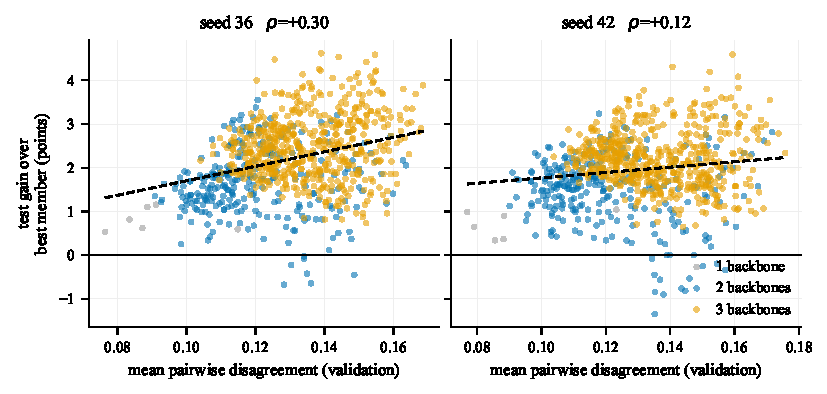
\includegraphics[width=0.84\textwidth]{fig3_diversity.pdf}
\caption{All 816 three-model ensembles per seed. Disagreement is measured on
validation, the gain on test, so no test information enters the horizontal
axis. Triples spanning three backbones (orange) sit systematically above those
built from a single backbone (grey). Mean member accuracy, not shown, carries
almost none of this signal on its own (Table~\ref{tab:reg}).}
\label{fig:diversity}
\end{figure}

\paragraph{What explains the gain.}
Fig.~\ref{fig:diversity} plots every triple. To separate the two candidate
explanations we regress the gain over the best member on the mean member
accuracy, on the mean pairwise disagreement, and on both (Table~\ref{tab:reg}).

\begin{table}[tb]
\centering
\caption{Linear models for the \emph{test} gain of an ensemble over its best
member, with both predictors measured on \emph{validation}. Fitted over all 816
triples per seed; $p$-values in parentheses.}
\label{tab:reg}
\begin{tabular}{llrrr}
\toprule
Seed & Predictors & mean acc. (val) & disagreement (val) & $R^2$ \\
\midrule
\multirow{3}{*}{36}
 & mean accuracy & $+0.031$ \, ($0.29$) & --- & 0.001 \\
 & disagreement  & --- & $+16.56$ \, ($1\!\times\!10^{-20}$) & 0.101 \\
 & both          & $+0.559$ \, ($1\!\times\!10^{-43}$) & $+43.28$ \, ($3\!\times\!10^{-62}$) & 0.290 \\
\midrule
\multirow{3}{*}{42}
 & mean accuracy & $+0.153$ \, ($2\!\times\!10^{-10}$) & --- & 0.049 \\
 & disagreement  & --- & $+6.13$ \, ($4\!\times\!10^{-5}$) & 0.021 \\
 & both          & $+0.713$ \, ($9\!\times\!10^{-80}$) & $+42.03$ \, ($1\!\times\!10^{-74}$) & 0.369 \\
\bottomrule
\end{tabular}
\end{table}

On its own, mean member accuracy explains essentially nothing about how much an
ensemble gains: $R^2 = 0.001$ under seed 36, with the coefficient not
significant ($p = 0.29$). Under seed 42 it reaches $R^2 = 0.049$, still small.
Disagreement on its own does better under seed 36 and worse under seed 42, so
neither single-predictor model is dependable.

The joint model is. Under both seeds $R^2$ rises sharply --- to 0.29 and 0.37
--- and the disagreement coefficient is large and highly significant
($+43.3$ and $+42.0$). The jump happens because the two predictors are mildly
negatively related: the most diverse triples tend to contain weaker members, so
each variable masks part of the other's effect until both are present. A
practitioner who ranks candidates by accuracy alone is looking at the predictor
that, on its own, carries almost no information about how much ensembling will
help.

\paragraph{Backbone diversity is a cheap proxy.}
Counting distinct backbones carries most of the same signal without computing
anything. Triples drawn from one backbone --- three heads on the same features
--- gain 0.77 and 0.57 points on average; spanning two backbones gains 1.61 and
1.43, and spanning three gains 2.42 and 2.20. Architectural variety does the
work that independent random seeds are usually asked to do, at no extra
training cost.

\section{Choosing Ensemble Members}
\label{sec:select}

Table~\ref{tab:strategy} compares selection rules a practitioner could actually
apply. Every rule sees only the validation split; the reported accuracy is on
test, and the gain is over the test accuracy of the single model that
validation nominates as best. That model is EfficientNetV2B0 with
DUAL\_POOLING\_FC under both seeds, reaching 90.71\% and 90.43\% on test.

\begin{table}[tb]
\centering
\caption{Ensemble member selection rules, applied using validation data only
and scored on test. Gain is over the test accuracy of the single model
validation ranks first. The oracle row is the best of all 816 triples on test
and is not a usable rule.}
\label{tab:strategy}
\begin{tabular}{lrrrr}
\toprule
& \multicolumn{2}{c}{seed 36} & \multicolumn{2}{c}{seed 42} \\
\cmidrule(lr){2-3}\cmidrule(lr){4-5}
Selection rule (validation only) & acc. & gain & acc. & gain \\
\midrule
Three most accurate models               & 92.62 & $+1.91$ & 92.45 & $+2.03$ \\
Most accurate per backbone               & 92.57 & $+1.86$ & 93.19 & $+2.76$ \\
Most disagreeing triple overall          & 91.92 & $+1.21$ & 91.39 & $+0.96$ \\
Most disagreeing within 2 points of best & 92.40 & $+1.69$ & 92.51 & $+2.08$ \\
Random triple (mean of 200)              & 91.80 & $+1.09$ & 91.69 & $+1.26$ \\
\midrule
Oracle on test (not usable)              & 93.38 & $+2.67$ & 93.36 & $+2.93$ \\
\bottomrule
\end{tabular}
\end{table}

\paragraph{Maximising diversity does not survive an honest protocol.}
This is the result we did not expect, and it is worth stating plainly. When we
measured disagreement on the test set --- as the ensemble diversity literature
routinely does --- the rule "take the most disagreeing triple among members
within 2 points of the best" was the strongest usable rule by a clear margin,
gaining 3.72 and 3.27 points. Re-estimating exactly the same rule on validation
drops it to 1.69 and 2.08, at or below simply taking the three most accurate
models. About half of its apparent advantage was the selection rule fitting the
test set.

The underlying statistical relationship is not the problem: Table~\ref{tab:reg}
shows that validation-measured disagreement still predicts test gain strongly.
The problem is the sharpness of the rule. Picking the single
disagreement-maximising triple out of 816 candidates is a high-variance
decision, and the disagreement estimate carries enough noise from a 3{,}511-image
validation split that the argmax often lands on a triple whose diversity was
overstated. A statistically real signal does not automatically give a reliable
selection rule, and reporting the rule without the honest protocol would have
overstated what a practitioner can expect by roughly two points.

\paragraph{What does survive is structural.}
Taking the most accurate model from each of three different backbones needs no
diversity estimate at all, only the identity of the architectures. It reaches
93.19\% under seed 42, beating the three-most-accurate rule by 0.74 points, and
92.57\% under seed 36, losing to it by 0.05. It beats a random triple by 0.77
and 1.50 points. Because it reads nothing off the validation predictions beyond
a per-model accuracy ranking, there is very little for it to overfit.

\paragraph{The rule holds at every ensemble size.}
Our choice of three members was a convenience, so we repeated the comparison
for $k = 2,\dots,6$ under the same validation-only protocol
The point of the sweep is robustness rather than tuning: taking one model per
backbone beats a random selection of the same size at all five sizes under both
seeds, ten comparisons out of ten, by between 0.6 and 1.5 points. The advantage
of spanning architectures is not an artefact of the ensemble size we happened
to pick.

Whether more than three members is worth the inference cost is less clear.
Moving from $k=3$ to $k=4$ gains 0.79 points under seed 36 but only 0.08 under
seed 42, and the curves are flat from $k=4$ onwards. That asymmetry is worth
unpacking, because it is not about ensemble size at all. Under seed 36 the
third- and fourth-ranked backbones are separated by 0.09 points of validation
accuracy, and the one that wins that near-tie, ResNet50, is the weaker partner:
substituting Xception for it at $k=3$ raises test accuracy from 92.57\% to
93.33\%. Under seed 42 the same two backbones are 0.43 points apart, Xception
wins, and $k=3$ is already strong. The jump at $k=4$ is the cost of a coin-flip
between two near-tied candidates, recovered one step later by admitting the
backbone that should have been third --- the same high-variance selection
problem that defeats the diversity-maximising rules, in a different place. We
therefore draw no recommendation about ensemble size.

\section{Limitations}
\label{sec:limits}

Two seeds per configuration bound run-to-run variation but do not estimate it
well. Statements we make about replication mean "held under both seeds", not
"significant across seeds"; a proper variance estimate would need at least five.
Where a difference in Table~\ref{tab:main} is smaller than the seed-to-seed
spread for the same configuration, we have deliberately refrained from ranking.

All results come from a single dataset. The head-capacity and diversity effects
have clear mechanisms that are not specific to waste imagery, but we have not
shown that the numbers transfer, and the magnitude of the diversity effect
plausibly depends on how fine-grained the label set is. A replication on a
second long-tailed, fine-grained benchmark is the obvious next step.

We use unweighted soft voting throughout. Learned combination weights would
likely raise the absolute numbers, and could plausibly change which selection
rule wins, since weighting partly compensates for a badly chosen member. We
sweep the ensemble size from two to six but do not go further, because six
backbones is the pool we trained.

Our validation split has 3{,}511 images, and Section~\ref{sec:select} shows that
the noise in a diversity estimate from a split of that size is enough to blunt
an argmax-style selection rule. With a larger validation split, or diversity
estimated by cross-validation on the training set, the diversity-maximising
rules might recover some of the advantage they show when diversity is measured
on test. We did not test this, and we would rather report the rule that worked
under the protocol we can defend.

\section{Conclusion}

We trained a complete 6$\times$3 grid of backbones and classifier heads twice on
a 36-class fine-grained waste dataset and analysed per-image predictions rather
than summary scores. The classifier head turned out to be the more dependable
design axis: its effect held on every backbone under both seeds, while the
backbone ranking changed between seeds. Head capacity bought training accuracy
and not test accuracy, with the train--test gap rising monotonically from 3.6 to
7.3 points.

More than a third of all model pairs were statistically indistinguishable by
McNemar's test, and those pairs still disagreed on roughly 12\% of the test set.
Across all 816 three-model ensembles, the mean accuracy of the members
explained almost none of the gain over the best member, while their pairwise
disagreement explained a great deal --- and this held with both predictors
measured on validation rather than on test.

The practical lesson is narrower than the statistical one, and the gap between
them is itself a finding. Selecting the most diverse triple looked like the
best rule available while diversity was estimated on the test set, and lost
about half its advantage once that estimate moved to validation. What survived
was the rule that needs no estimate at all: take the best model from each of
several different backbones. That rule beat a random selection of the same size
at every ensemble size we tried, under both seeds. Architectural variety buys
most of the available diversity without asking a noisy statistic to pick the
winner.

The broader methodological point is that the per-image predictions of an
experiment already run contain considerably more information than the table
usually published from them --- including, as here, enough to catch a
conclusion that would not have replicated.

% TODO TRUOC KHI NOP: tao repo va thay URL that vao day.
\paragraph{Reproducibility.}
All 36 models were trained in public Kaggle notebooks, which record the
environment, the random seeds and the full training logs. We release the
per-image predictions of every model on both the validation and the test
split --- the validation predictions are what make the selection protocol of
Section~\ref{sec:select} checkable --- together with the
analysis scripts that produce each number, table and figure in this paper, so
that the grid need not be retrained to check any result. Materials are
available at \url{https://github.com/REPO-TODO}.

\bibliographystyle{splncs04}
\bibliography{references}

\end{document}
